
\chapter{Examples of Finite Elements}\label{chap4}

WE\pageoriginale SUMMARIZE BELOW {\em our requirements regarding the
  ``finite element subspaces''} $V_{h}$
\begin{enumerate}
\renewcommand{\theenumi}{\roman{enumi}}
\renewcommand{\labelenumi}{(\theenumi)}
\item Let $\Omega\subset \mathbb{R}^{n}$ be a polygonal domain. Let
  $\mathfrak{k}_{h}$ be a triangulation of $\Omega$ as in
  Sec.~\ref{chap3}. Then $V_{h}$ is a finite-dimensional vector space
  such that for all $v\in V_{h}$, $v|K\in P_{K}$ for every finite
  element $K$, where $P_{K}$ is a vector space of finite
  dimension. Usually, $P_{K}$ {\em is a space of polynomials}. This is
  of practical importance in computing the matrix of the system. We
  shall see later that it is of theoretical importance as
  well. Observe for the moment that if $P_{K}$ consists of
  polynomials, then we automatically have that $P_{K}\subset H^{1}(K)$
  or $P_{K}\subset H^{2}(K)$. 

\item By Theorem \ref{chap3-thm3.2}, $V_{h}\subset
  C^{0}(\overline{\Omega})$ implies that $V_{h}\subset H^{1}(\Omega)$
  and by Exercise \ref{chap3-exer3.1} $V_{h}\subset
  C^{1}(\overline{\Omega})$ implies that $V_{h}\subset
  H^{2}(\Omega)$. Thus we must choose a {\em proper basis for the
    ``local'' spaces $P_{K}$ such that these ``global'' inclusions
    hold.}

\item {\em There must exist at least one basis $\{w_{j}\}$ of $V_{h}$
  which consists of functions with ``small'' support.}
\end{enumerate}

We bear these points in mind when constructing examples of finite
elements. Before we proceed we need a few definitions.

\begin{definition}\label{chap4-defi4.1}
An $n$-simplex is the convex hull in $\mathbb{R}^{n}$ of $(n+1)$
points $\{a_{j}\}^{n+1}_{j=1}$ such that if $a_{j}=(a_{kj})^{n}_{k=1}$
and $A$ is the matrix
\begin{equation*}
A=
\begin{pmatrix}
a_{11} & a_{12} & \ldots & a_{1,n+1}\\
\vdots & \vdots & & \vdots\\
a_{n1} & a_{n2} & \ldots & a_{n,n+1}\\
1 & 1 & \ldots & 1
\end{pmatrix}\tag{4.1}\label{chap4-eq4.1}
\end{equation*}
then\pageoriginale $\det A\neq 0$.
\end{definition}

The above definition generalises the notion of a triangle to $n$
dimensions. Geometrically the condition $\det A\neq 0$ simply means
that the points $\{a_{j}\}^{n+1}_{j=1}$ do not lie in the same
hyperplane. For $\det A$ is equal to, by elementary column operations,
the determinant of the matrix
$$
\begin{pmatrix}
(a_{11}-a_{1,n+1}) & \ldots & (a_{1,n}-a_{1,n+1})\\
\vdots & & \vdots\\
(a_{n1}-a_{n,n+1}) & \ldots & (a_{n,n}-a_{n,n+1})
\end{pmatrix}
$$
and that this is non-zero means that
$(a_{1}-a_{n+1}),\ldots,(a_{n}-a_{n+1})$ are linearly independent
vectors in $\mathbb{R}^{n}$, which is the same as saying that
$a_{1},\ldots,a_{n+1}$ do not lie in the same hyperplane.

\begin{definition}\label{chap4-defi4.2}
Let $\{a_{j}\}^{n+1}_{j=1}$ be $(n+1)$-points in $\mathbb{R}^{n}$
satisfying the conditions of definition \ref{chap4-defi4.1}. The
barycentric coordinates of any $x\in \mathbb{R}^{n}$ with respect to
these points are numbers $\{\lambda_{j}\}^{n+1}_{j=1}$ such that
\begin{equation*}
\begin{cases}
x=\sum\limits^{n+1}_{j=1}\lambda_{j}a_{j},\\
1=\sum\limits^{n+1}_{j=1}\lambda_{j}.
\end{cases}\tag{4.2}\label{chap4-eq4.2}
\end{equation*}
\end{definition}

The barycentric coordinates exist because they are merely the
components of the unique solution vector $\overrightarrow{\lambda}$ of
the system of $(n+1)$ linear equations in $(n+1)$ unknowns given by
\begin{equation*}
A\overrightarrow{\lambda}=\binom{\ora{x}}{1}\quad\text{where}\quad
\ora{x}=
\begin{pmatrix}
x_{1}\\
\vdots\\
x_{n}
\end{pmatrix}
\end{equation*}

The functions $\lambda_{j}=\lambda_{j}(x)$ are all affine functions of
$x$. Also $\lambda_{j}(a_{i})=\delta_{ij}$,\pageoriginale where
$\delta$ is the Kronecker symbol.

\begin{remark}\label{chap4-rem4.1}
Given points $\{a_{j}\}^{n+1}_{j=1}$ as in the definition
\eqref{chap4-eq4.1}, the corresponding $n$-simplex is given by
$$ 
K=\left\{x=\sum\limits^{n+1}_{j=1}\lambda_{j}a_{j};\ 0\leq
\lambda_{j}\leq 1;\ \sum\limits^{n+1}_{j=1}\lambda_{j}=1\right\}. 
$$
\end{remark}

\begin{definition}\label{chap4-defi4.3}
Let $k\geq 0$ be an integer. Then, $P_{k}$ is the space of all
polynomials of degree $\leq k$ in $x_{1},\ldots,x_{n}$.
\end{definition}

We now proceed with {\em examples of finite elements.}

\begin{example}\label{chap4-exam4.1}
The $n$-simplex of type $(1)$.
\end{example}

Let $K$ be an $n$-simplex. Let $P_{K}=P_{1}$. We define a set
$\sum_{K}=\{p(a_{i}); 1\leq i\leq n+1\}$ {\em of degrees of freedom}
for $p\in P_{K}$, where $\{a_{i}\}^{n+1}_{i=1}$ are the vertices of
$K$: {\em The set $\sum_{K}$ determines every polynomial $p\in P_{K}$
  uniquely.} For, note that $\dim P_{K}=\dim P_{1}=n+1$. Consider
$\lambda_{1},\ldots,\lambda_{n+1}\in P_{1}$, the barycentric
coordinate functions. These are linearly independent since $\sum
\alpha_{k}\lambda_{k}=0$ implies that its value at each vertex is
zero. Since $\lambda_{k}(a_{j})=\delta_{kj}$ we get that
$\alpha_{j}=0$ for all $j$. Thus these functions form a basis for
$P_{1}$. Let us write
$$
p=\sum^{n+1}_{i=1}\alpha_{i}\lambda_{i}.
$$ 

Then
$$
p(a_{j})=\sum^{n+1}_{i=1}\alpha_{i}\lambda_{i}(a_{j})=\sum^{n+1}_{i=1}\alpha_{i}\delta_{ij}=\alpha_{j}. 
$$

Thus,
\begin{equation*}
p=\sum^{n+1}_{i=1}p(a_{i})\lambda_{i}.\tag{4.4}\label{chap4-eq4.4} 
\end{equation*}

\begin{example}\label{chap4-exam4.2}
The $n$-simplex of type (2).


Let\pageoriginale $K$ be an $n$-simplex with vertices
$\{a_{i}\}^{n+1}_{i=1}$. Let 
$a_{ij}(i<j)$ be the mid-points of the line joining $a_{i}$ and
$a_{j}$, i.e.\@ $a_{ij}=\frac{1}{2}(a_{i}+a_{j})$. 
\begin{figure}[H]
\centering
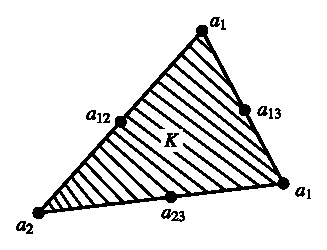
\includegraphics{figure/fig4.1.eps}
\caption{}\label{chap4-fig4.1}
\end{figure}

Let $P_{K}=P_{2}$. We define for $p\in P_{2}$, {\em the set}
$\sum_{K}=\{p(a_{i}), 1\leq i\leq n+1; p(a_{ij}), 1\leq i<j\leq n+1\}$
{\em of degrees of freedom.} Again $\sum_{K}$ determines $p\in P_{2}$
completely. To see this note that $\dim P_{K}=\binom{n+2}{2}$ and
there are as many functions in the set $\{\lambda_{i}(2\lambda_{i}-1),
1\leq i\leq n+1; \lambda_{i}\lambda_{j},1\leq i\leq j\leq
n+1\}$. There are all functions in $P_{2}$. Further since
$$ 
\lambda_{i}(a_{j})=\delta_{ij},\ \lambda_{i}(a_{kj})=
\begin{cases}
\frac{1}{2}\text{~ if~ } i=k\text{~ or~ }j,\\
0\quad \text{otherwise,}
\end{cases}
$$
we see again that these are linearly independent in $P_{2}$. Let us
write
$$
p=\sum^{n+1}_{i=1}\alpha_{i}\lambda_{i}(2\lambda_{i}-1)+\sum_{1\leq
  i<j\leq n+1}\beta_{ij}\lambda_{i}\lambda_{j}.
$$

Then 
$$
p(a_{k})=\sum^{n+1}_{i=1}\alpha_{i}\delta_{ik}(2\delta_{ik}-1)=\alpha_{k}.
$$

Further,
\begin{align*}
p(a_{kl}) &=
\sum^{n}_{i=1}\alpha_{i}(2\lambda^{2}_{i}(a_{kl})-\lambda_{i}(a_{kl}))\\ 
&\quad +\sum_{1\leq i<j\leq
  n+1}\beta_{ij}\lambda_{i}(a_{kl})\lambda_{j}(a_{kl}). 
\end{align*}

But\pageoriginale since $\lambda_{i}(a_{kl})=0$ or $\frac{1}{2}$, the
first sum $\sum\limits^{n}_{i=1}$ is zero. Further,
$$
\lambda_{i}(a_{kl})\lambda_{j}(a_{kl})=
\begin{cases}
\frac{1}{4}\text{~ if~ } (i,j)=(k,l)\text{~ or~ }(l,k),\\
0\quad\text{otherwise.}
\end{cases}
$$

Hence $\beta_{kl}=4p(a_{kl})$. Thus we have
\begin{equation*}
p=\sum^{n+1}_{i=1}\lambda_{i}(2\lambda_{i}-1)p(a_{i})+\sum_{1\leq
  i<j\leq
  n+1}4\lambda_{i}\lambda_{j}p(a_{ij}).\tag{4.5}\label{chap4-eq4.5} 
\end{equation*}
\end{example}

\begin{example}\label{chap4-exam4.3}
The $n$-simplex of type (3).

Let $K$ be an $n$-simplex with vertices $\{a_{i}\}^{n+1}_{i=1}$. Let
$a_{iij}=\dfrac{2a_{i}+a_{j}}{3}$, $i\neq j$. Let
$a_{ijk}=\dfrac{a_{i}+a_{j}+a_{k}}{3}$ for $i<j<k$.
\begin{figure}[H]
\centering
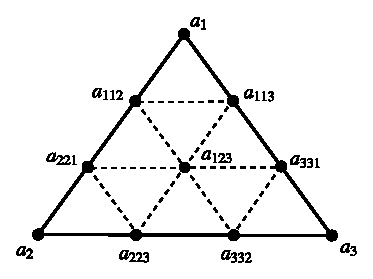
\includegraphics{figure/fig4.2.eps}
\caption{}\label{chap4-fig4.2}
\end{figure}

Set $P_{K}=P_{3}$. Define {\em the set of degrees of freedom}
\begin{align*}
\sum_{K} & =\left\{p(a_{i}),1\leq i\leq n+1;\ p(a_{iij}),\ 1\leq i\neq
j\leq n+1; \right. \\
&  \hspace{3.7cm}\left.  p(a_{ijk}),\ 1\leq i<j<k\leq a+1\right\}.
\end{align*}

Note that $\lambda_{i}(a_{iij})=\dfrac{2}{3}$;
$\lambda_{j}(a_{iij})=\dfrac{1}{3}$; $\lambda_{1}(a_{iij})=0$ if
$1\neq i$, $1\neq j$; $\lambda_{1}(a_{ijk})=\dfrac{1}{3}$ if $1=i,j$
or $k$ and $0$ otherwise, etc. Using these, one checks the linear
independence of the functions
\begin{align*}
&  \left\{\lambda_{i}(3\lambda_{i}-1)(3\lambda_{i}-2),\ 1\leq i\leq
n+1;\ \lambda_{i}\lambda_{j}(3\lambda_{i}-1),\ 1\leq i\neq j\leq
n+1; \right.\\
& \hspace{6cm} \left.  \lambda_{i}\lambda_{j}\lambda_{k}1\leq i<j<k\leq n+1\right\}.
\end{align*}

These then form a basis for $P_{3}$, for there are as many functions
in the above collection as $\dim P_{K}$. Using the values of
$\lambda_{i}$ at the special points described above, we get
\begin{equation*}
\begin{split}
p &=
\sum^{n+1}_{i=1}\frac{\lambda_{i}(3\lambda_{i}-1)(3\lambda_{i}-2)}{2}p(a_{i})\\
&\quad + \sum_{1\leq i\neq j\leq
  n+1}\frac{9}{2}\lambda_{i}\lambda_{j}(3\lambda_{i}-1)p(a_{iij})\\ 
&\quad \sum_{1\leq i<j<k\leq
  n+1}27\lambda_{i}\lambda_{j}\lambda_{k}p(a_{ijk}). 
\end{split}\tag{4.6}\label{chap4-eq4.6}
\end{equation*}\pageoriginale

Thus $\sum_{K}$ completely determines $p\in P_{3}$.
\end{example}

The points of $K$ at which the polynomials are evaluated to get
$\sum_{K}$ are known as the {\em nodes of the finite element}. The set
$\sum_{K}$ is the set of {\em degrees of freedom of the finite
  element.}

\begin{exercise}\label{chap4-exer4.1}
Generalize these ideas and describe the $n$-{\em simplex of type
  $(k)$} for any integer $k\geq 1$. 
\end{exercise}

We now show how these finite elements may be used to define the space
$V_{h}$.

First of all we show the inclusion $V_{h}\subset
C^{0}(\overline{\Omega})$. Consider for instance a triangulation by
$n$-simplices of type (1). Number all the nodes of the triangulation
by $\{b_{j}\}$. Let us define $\sum_{h}=\{p(b_{j});\ b_{j}\text{~ is a
  node.}\}$: This is the {\em set of degrees of freedom of the space}
$V_{h}:A$ function $v$ in the space $V_{h}$ is, by definition,
determined over each $K\in\mathfrak{k}_{h}$ by the values $v(b_{j})$
for those nodes $b_{j}$ which belong to $K$.

Let us examine the two-dimensional case, for simplicity. If $K_{1}$
and $K_{2}$ are two adjacent triangles with common side $K'$
(cf. Fig.~\ref{chap4-fig4.3}), we need to show that $v|K_{1}=v|K_{2}$
along $K'$ for any $v\in V_{h}$. Let $t$ be an abscissa along $K'$.
\begin{figure}[H]
\centering
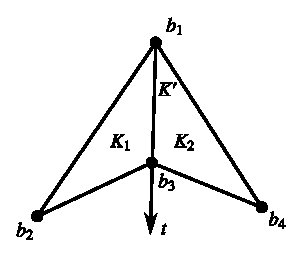
\includegraphics{figure/fig4.3.eps}
\caption{}\label{chap4-fig4.3}
\end{figure}\pageoriginale 

Now $v|K_{1}$ along $K'$ is a polynomial of degree $1$ in $t$. So is
$v|K_{2}$ along $K'$. But {\em these two agree at the nodes $b_{1}$
  and $b_{3}$}. Therefore, they must be identical and hence the
continuity of $v$ follows.

This argument can be extended to any simplex of type $(k)$. These
simplices, by Theorem \ref{chap3-thm3.2} yield the inclusion
$V_{h}\subset H^{1}(\Omega)$ and hence we may use them for second
order problems.

\begin{exercise}\label{chap4-exer4.2}
The triangle of type $(3')$.

Let $K$ be a triangle in $\mathbb{R}^{2}$. Define $\sum_{K}$ to be the
values of $p$ at the points $\{a_{i},1\leq i\leq 3\}$, and the points
$\{a_{iij},1\leq i\neq j\leq 3\}$. If we define $P'_{3}=\{p\in P_{3};
12p(a_{123})+2\sum^{3}_{i=1}p(a_{i})-3\sum_{i\neq j}p(a_{iij})=0\}$,
then show that $\sum_{K}$ uniquely determines $p\in
P'_{3}=P_{K}$. Further show that $P_{2}\subset P'_{3}$.
\end{exercise}

We now relax our terminological rules about ``triangulations'' and
admit rectangles (and in higher dimensions, hyper rectangles or
hypercubes) in triangulations. We describe below some finite elements
which are rectangles.

We need another space of polynomials.

\begin{definition}\label{chap4-defi4.4}
Let $k\geq 1$ be an integer. Then 
$$
Q_{k}=\left\{p;p(x)=\sum_{\substack{0\leq i_{j}\leq k\\ 1\leq j\leq
    n}}a_{i_{1},\ldots i_{n}}x^{i_{1}}_{1}\ldots x^{i_{n}}_{n}\right\}.
$$\pageoriginale
\end{definition}

We have the inclusions $P_{k}\subset Q_{k}\subset P_{nk}$.

\begin{example}\label{chap4-exam4.4}
The Rectangle of type $(1)$.

Let $K$ be the unit square in $\mathbb{R}^{2}$, i.e.,
$K=[0,1]^{n}$. Let $P_{K}=Q_{1}$. The set of degrees of freedom is
given by $\sum_{K}=\{p(a_{i}),1\leq i\leq 4\}$;
cf. Fig.~\ref{chap4-fig4.4} in the case $n=2$. 
\begin{figure}[H]
\centering
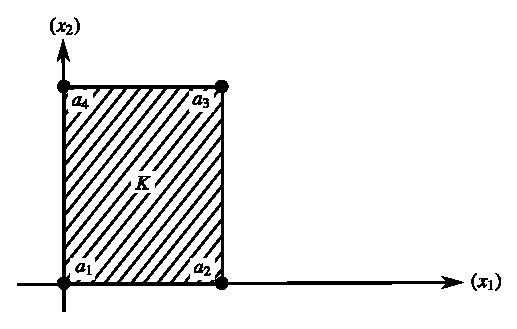
\includegraphics{figure/fig4.4.eps}
\caption{}\label{chap4-fig4.4}
\end{figure}

To show that $\sum_{K}$ indeed determines $p\in Q_{1}$ uniquely we
adopt a different method now. (There are essentially two methods to
show that $\sum_{K}$ completely determines $P_{K}$; the first was used
in the previous examples where we exhibited a basis for $P_{K}$ such
that the corresponding coefficients in the expansion of $p$ in terms
of this basis came from $\sum_{K}$; the second is illustrated now).

Observe first that $\dim P_{K}=\card \sum_{K}=2^{n}$. To determine a
polynomial completely in terms of the elements of $\sum_{K}$ we must
solve $2^{n}$ linear equations in as many unknowns. That every
polynomial is determined this way is deduced from the existence of a
solution to this system. But for such a system\pageoriginale the
existence and uniqueness of the solution are equivalent, and one
establishes the latter. Thus we show that if $p\in P_{K}$ such that
all its degrees of freedom are zero, the $p\equiv 0$.

Returning to our example, consider a polynomial $p\in Q_{1}$ such that
$p(a_{i})=0$ for all $1\leq i\leq 4$. On each side $p$ is a polynomial
of degree $1$ either in $x_{1}$ alone or in $x_{2}$ alone. Since it
vanishes at two points, the polynomial $p$ vanishes on the sides of
the square. Now consider various lines parallel to one of the
axes. Here too $p$ is a polynomial of degree $1$ in one variable
only. Since it vanishes at the points where the line meets the side,
it also vanishes on this line. Varying the line we get $p\equiv
0$\footnote[1]{It is not necessary to restrict ourselves to a
  square. Any rectangle with sides parallel to the coordinate axes
  would do.}.  
\end{example}


\begin{example}\label{chap4-exam4.5}
The Rectangle of type (2).

Again consider the unit square (or hypercube in $\mathbb{R}^{n}$) to
be the finite element $K$. Set $P_{K}=Q_{2}$, and
$\sum_{K}=\{p(a_{i}),1\leq i\leq 9\}$ where the $a_{i}$ are as in the
figure below.
\begin{figure}[H]
\centering
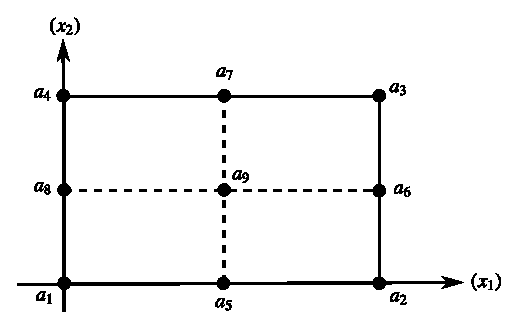
\includegraphics{figure/fig4.5.eps}
\caption{}\label{chap4-fig4.5}
\end{figure}

Here again one can prove the unisolvency as above. Now let $p\in
Q_{2}$ be given such that $p(a_{i})=0$ for all $1\leq i\leq 9$; then
$p=0$ on the four sides and on the two central (dotted, in
Fig.~\ref{chap4-fig4.5}) lines. Now take lines parallel to one
of\pageoriginale the axis and $p$ vanishes on each of these. Thus
$p\equiv 0$ on $K$ and we get that $\sum_{K}$ uniquely determines
$p\in Q_{2}$.
\end{example}

\begin{exercise}\label{chap4-exer4.3}
Describe the rectangle of type (3) and generalize to hyper-rectangles
of type $(k)$.
\end{exercise}

\begin{exercise}\label{chap4-exer4.4}
Prove that in all the preceding examples, we get $V_{h}\subset C^{0}(\Omega)$.
\end{exercise}

\begin{exercise}\label{chap4-exer4.5}
The Rectangle of type $(2')$.


Let $K$ be as in example \ref{chap4-exam4.5}. However omit the node
$a_{9}$ (the centroid of $K$). Let $\sum_{K}=\{p(a_{i}),1\leq i\leq
8\}$ and show that this determines uniquely a function in the space
$$
P_{K}=\left\{p\in Q_{2};
4p(a_{9})+\sum^{4}_{i=1}p(a_{i})-2\sum^{8}_{i=5}p(a_{i})=0\right\}. 
$$
and that $P_{2}\subset P_{K}$.
\end{exercise}

We now turn to different types of finite elements. They differ from
the preceding ones in the choice of degrees of freedom as will be seen
presently. 

\begin{example}\label{chap4-exam4.6}
The Hermite Triangle of Type (3).

Let $K\subset \mathbb{R}^{2}$ be a triangle with vertices
$\{a_{1},a_{2},a_{3}\}$. Let $\lambda_{i},1\leq i\leq 3$, be the
barycentric coordinate functions. Then one can check that any
polynomial $p\in P_{3}=P_{K}$ can be expanded as
\begin{align*}
p &=
\sum^{3}_{i=1}(-2\lambda^{3}_{i}+3\lambda^{2}_{i}-7\lambda_{1}\lambda_{2}\lambda_{3})p(a_{i})+27\lambda_{1}\lambda_{2}\lambda_{3}p(a_{123})\\
&\quad +\sum^{3}_{i=1}\sum_{\substack{j=1\\ j\neq
    i}}\lambda_{i}\lambda_{j}(2\lambda_{i}+\lambda_{j}-1)\Dp(a_{i})(a_{j}-a_{i}). 
\end{align*}

Thus, $\sum_{K}=\{p(a_{i}),1\leq i\leq 3;\Dp
(a_{i})(a_{j}-a_{i}),1\leq i\neq j\leq 3;p(a_{123})\}$ is the
corresponding set of degrees of freedom.

Note\pageoriginale that $\Dp(a_{i})$ is the Frechet derivative of $p$
evaluated at $a_{i}$: If $(e_{1},\ldots,e_{n})$ is the standard basis
for $\mathbb{R}^{n}$, then for $v:\mathbb{R}^{n}\to R$, we have,
$(\Dv)(x)(e_{i})=\dfrac{\p v}{\p x_{i}}(x)$, the usual partial
derivative.

Notice that we may replace $\sum_{K}$ by the set
$$
\sum'_{K}=\left\{p(a_{i}),1\leq i\leq 3; p(a_{123});\frac{\p p}{\p
  x_{1}}(a_{i}), \frac{\p p}{\p x_{2}}(a_{i}), 1\leq i\leq 3\right\}.
$$
\end{example}

\begin{remark}\label{chap4-rem4.2}
The term ``{\em Hermite}'' means that we assume knowledge of
derivatives at some of the nodes. If only the values of $p$ at the
nodes appear in the set of degrees of freedom, as was the case upto
Example \ref{chap4-exam4.5}, we refer to the finite elements as of
``{\em Lagrange}'' type. These ideas will be made precise in
Sec.~\ref{chap5}. We usually indicate degrees of freedom involving
derivatives by circling the nodes - one circle for first derivatives,
two for first and second derivatives and so on. Thus the finite
element of example \ref{chap4-exam4.6} may be pictured as in
Fig.~\ref{chap4-fig4.6}. 
\begin{figure}[H]
\centering
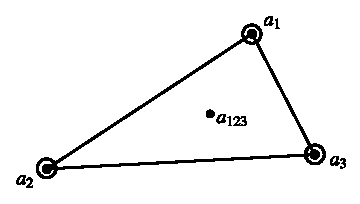
\includegraphics{figure/fig4.6.eps}
\caption{}\label{chap4-fig4.6}
\end{figure}
\end{remark}

\begin{exercise}\label{chap4-exer4.6}
The Hermite Triangle of Type $(3')$.

This is also known as the {\em Zienkiewicz triangle} in Engineering
literature. Set $\sum_{K}=\left\{p(a_{i}),\dfrac{\p p}{\p
  x_{1}}(a_{i}), \dfrac{\p p}{\p x_{2}}(a_{i}),1\leq i\leq
3\right\}$. Show that $\sum_{K}$ uniquely determines a function in the
space
$$
P_{K}=\left\{p\in
P_{3};\ 6p(a_{123})-2\sum^{3}_{i=1}p(a_{i})+\sum^{3}_{i=1}Dp(a_{i})(a_{i}-a_{123})=0\right\}. 
$$
\end{exercise}

All\pageoriginale examples cited upto now yield the inclusion
$V_{h}\subset C^{0}(\overline{\Omega})$ and consequently are useful to
solve second-order problems. In order to solve problems of fourth
order, we need the inclusion $V_{h}\subset
C^{1}(\overline{\Omega})$. Our subsequent examples will be in this
direction. 

\begin{remark}\label{chap4-rem4.3}
Consider a $1$-simplex $K\subset \mathbb{R}^{1}$. A triangulation is
merely a subdivision of $\Omega$ into subintervals. In any subinterval
$K$ not only $v|K$ but also $\dfrac{d(v|K)}{dx}$ must be continuous at
both end points. Thus we get 4 conditions on $v|K$. Consequently
$P_{K}$ must contain all polynomials of degree 3 in it. The analogous
result (which is non-trivial) is due to A. \v{Z}eni\v{s}ek
\cite{key24} that is case of $\mathbb{R}^{2}$, and $K$ a triangle of
$\mathbb{R}^{2}$, at least polynomials of degree 5 must be contained in
  $P_{K}$. 

\end{remark}

\begin{example}\label{chap4-exam4.7}
The Argyris triangle.

This is also known as the {\em 21-degree-of-freedom-triangle.} We set
$P_{K}=P_{5}$ and
\begin{gather*}
\sum_{K}=\left\{p(a_{i}),\dfrac{\p p}{\p
  x_{1}}(a_{i}),\ldots,\dfrac{\p^{2}p}{\p x^{2}_{2}}(a_{i}),\ 1\leq
i\leq 3;\right.\\
\left. \dfrac{\p p}{\p \nu}(a_{ij}),\ 1\leq i\leq j\leq 3\right\}.
\end{gather*}
\begin{figure}[H]
\centering
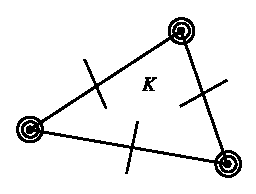
\includegraphics{figure/fig4.7.eps}
\caption{}\label{chap4-fig4.7}
\end{figure}

The\pageoriginale knowledge of the normal derivative $\dfrac{\p p}{\p
  \nu}$ is indicated by a line perpendicular to the side at the
appropriate point; cf.\@ Fig.~\ref{chap4-fig4.7}.

We now show that any $p\in P_{K}$ is uniquely determined by
$\sum_{K}$. Let $p\in P_{K}=P_{5}$ be given such that all its degrees
of freedom are zero. If $K'$ is any side of $K$ and $t$ is an abscissa
along $K'$ then $p|K'$ is a polynomial $p_{1}(t)$ of degree 5. The
vanishing of $p$, $\dfrac{dp}{dt}$, $\dfrac{d^{2}p}{dt^{2}}$ at the
end points, say $b$, $b'$, of $K'$ imply that all the 6 coefficients
of $p_{1}$ are $0$ and hence $p_{1}\equiv 0$. Thus
$p=0=\dfrac{dp}{dt}$ on $K'$. The polynomial $r(t)=\dfrac{\p p}{\p
  \nu}(t)$ is of degree $4$ on $K'$ and we also have
$r(b)=r(b')=\dfrac{dr}{dt}(b)=\dfrac{dr}{dt}(b')=r\left(\dfrac{b+b'}{2}\right)=0$
which imply that $r\equiv 0$ on $K'$. Hence $p$, $\dfrac{\p p}{\p
  x_{1}}$, $\dfrac{\p p}{\p x_{2}}$ all vanish on the sides of the
triangle $K$. The sides of $K$ are defined by the equations
$\lambda_{i}(x_{1},x_{2})=0$, $(i=1,2,3)$ where $\lambda_{i}$ are the
barycentric coordinate functions. We claim that $\lambda^{2}_{i}$
divides $p$ for $i=1,2,3$. To see this it is enough to prove that if
$p$ is a polynomial such that $p$, $\dfrac{\p p}{\p x_{1}}$,
$\dfrac{\p p}{\p x_{2}}$ vanish on any straight line
$L=\{(x_{1},x_{2});\lambda(x_{1},x_{2})=0\}$ then $\lambda^{2}$
divides $p$. In the special case, when $\lambda(x_{1},x_{2})=x_{1}$
writing $p(x_{1},x_{2})=\sum^{5}_{j=0}a_{j}(x_{2})x^{j}_{1}$ (with
deg.\@ $a_{j}\leq 5-j$) it follows that $a_{0}(x_{2})=a_{1}(x_{2})=0$
since $p=\dfrac{\p p}{\p x_{1}}=0$ on $L$. Thus $x^{2}_{1}$ divides
$p$. The general case reduces to this case by an affine
transformation. In fact, by translating the origin to a point $P$,
fixed arbitrarily on $L$ and by rotation of the coordinate axes we can
assume that $L=\{(X_{1},X_{2});X_{1}=0\}$ in the new coordinates. If
$p'$ is the image of $p$ under this transformation then $p'$ is also a
polynomial (of degree 5) and $p'$, $\dfrac{\p p'}{\p X_{1}}$,
$\dfrac{\p p'}{\p X_{2}}$ vanish on $L$ by chain rule for
differentiation. Hence $X^{2}_{1}$ divides $p'$. This is the same
thing as saying $\lambda^{2}$ divides $p$ which proves the
claim. Since $\lambda_{i}$ are mutually coprime we may now write
$p=q\lambda^{2}_{1}\lambda^{2}_{2}\lambda^{2}_{3}$. Then we
necessarily have $q(x_{1},x_{2})\equiv 0$ for, otherwise deg.\@ $p\geq
6$ which is impossible since $p\in P_{5}$. Hence $p\equiv 0$ on $K$
which proves that $\sum_{K}$ determines $p\in P_{5}$.

To define the corresponding space $V_{h}$, we number all the vertices
of the triangles by $\{b_{j}\}$ and all midpoints of the sides by
$\{c_{k}\}$. The {\em the set of degrees of\pageoriginale freedom of
  the space $V_{h}$ is}
$$
\sum_{h}=\left\{v(b_{j}),\frac{\p v}{\p x_{1}}(b_{j}),\frac{\p v}{\p
  x_{2}}(b_{j}),\frac{\p^{2}v}{\p x^{2}_{1}}(b_{j}),\frac{\p^{2}v}{\p
  x_{1}\p x_{2}}(b_{j}),\frac{\p^{2}v}{\p x^{2}_{2}}(b_{j}),\frac{\p
  v}{\p \nu_{k}}(c_{k})\right\} 
$$  
where $\dfrac{\p}{\p\nu_{k}}$ is one of the two possible normal
derivatives at the mid-point $c_{k}$.

We now show that $V_{h}\subset C^{1}(\overline{\Omega})$. Consider two
adjacent Argyris triangles $K_{1}$ and $K_{2}$ with common boundary
$K'$ along which $t$ is an abscissa (Fig.~\ref{chap4-fig4.8}). Let
$v\in V_{h}$. Now $v|K_{1}$ and $v|K_{2}$ are polynomials of degree
$5$ in $t$ along $K'$ and they agree together with their first and
second derivatives at the end points. Thus $v|K_{1}=v|K_{2}$ on $K'$,
proving continuity.

Now $\dfrac{\p(v|K_{1})}{\p\nu}$ and $\dfrac{\p(v|K_{2})}{\p \nu}$
along $K'$ are polynomials of degree $4$ agreeing in their values with
first derivatives at end points and agree at the mid-point in their
values. Thus $\dfrac{\p(v|K_{1})}{\p \nu}=\dfrac{\p(v|K_{2})}{\p \nu}$
on $K'$. Similarly, $\dfrac{\p (v|K_{1})}{\p t}=\dfrac{\p
  (v|K_{2})}{\p t}$ on $K'$ and hence $v\in
C^{1}(\overline{\Omega})$. Thus $V_{h}\subset
C^{1}(\overline{\Omega})$. 
\begin{figure}[H]
\centering
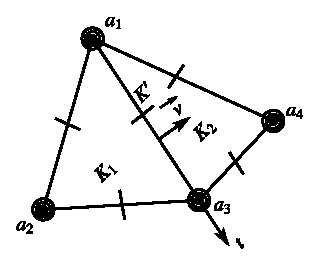
\includegraphics{figure/fig4.8.eps}
\caption{}\label{chap4-fig4.8}
\end{figure}
\end{example}

\begin{exercise}\label{chap4-exer4.7}
The $18$-Degree-of-Freedom-Triangle

Let $K$ be a triangle in $\mathbb{R}^{2}$. Let $P_{K}$ consist of
those polynomials of degree $\leq 5$ for which, along each side of
$K$, the normal derivative is a polynomial of degree $\leq 3$, in one
variable of course. Show that a polynomial in $P_{K}$ is uniquely
determined by the following set of degrees of freedom:
$$
\sum_{K}=\left\{p(a_{i}),\frac{\p p}{\p
  x_{1}}(a_{i}),\ldots,\frac{\p^{2}p}{\p x^{2}_{2}}(a_{i}),1\leq i\leq
3\right\}. 
$$\pageoriginale

Note that $P_{4}\subset P_{K}$ and $\dim P_{K}=18$.
\end{exercise}

\begin{exercise}\label{chap4-exer4.8}
The HCT-Triangle.

This element is due to Hsieh, Clough and Tocher. Let $a$ be any interior
point of the triangle $K$ with vertices $a_{1}$, $a_{2}$,
$a_{3}$. With $a$ as common vertex subdivide the triangle into
triangles $K_{1}$, $K_{2}$, $K_{3}$;
cf. Fig.~\ref{chap4-fig4.9}. Define
$$
P_{K}=\left\{p\in C^{1}(K);\ P|K_{i}\in P_{3},\ 1\leq i\leq 3\right\}.
$$

Obviously, $P_{3}\subset P_{K}$. The degrees of freedom are given by
$$
\sum_{K}=\left\{p(a_{i}),\frac{\p p}{\p x_{1}}(a_{i}), \frac{\p p}{\p
  x_{2}}(a_{i}),1\leq i\leq 3;\ \frac{\p p}{\p \nu}(a_{ij}),1\leq
i<j\leq 3\right\}.
$$
\begin{figure}[H]
\centering
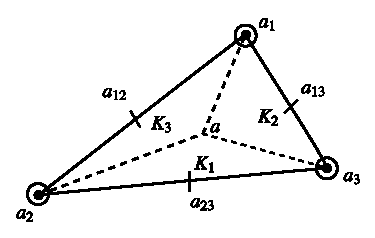
\includegraphics{figure/fig4.9.eps}
\caption{}\label{chap4-fig4.9}
\end{figure}

Show that $\sum_{K}$ uniquely determines $p\in P_{K}$.
\end{exercise}

\noindent
{\bf Note:}~ Since we have to determine 3 polynomials $p_{i}=p|K_{i}$
each of degree $\leq 3$, we need to determine 30 coefficients on the
whole. For this we have the following conditions:
\begin{itemize}
\item[(i)] The values at the vertices together with first derivatives
  and also the normal derivative at the mid points give 7 conditions
  for each $p_{i}=p|K_{i}$. Thus we have 21 conditions from these.

\item[(ii)] $p_{1}(a)=p_{2}(a)=p_{3}(a)$ gives 2 conditions.

\item[(iii)] $\dfrac{\p p_{1}}{\p x_{i}}(a)=\dfrac{\p p_{2}}{\p
  x_{i}}(a)=\dfrac{\p p_{3}}{\p x_{1}}(a)$\pageoriginale for $i=1,2$,
  gives 4 more conditions.

\item[(iv)] $\dfrac{\p p_{1}}{\p \nu}=\dfrac{\p p_{2}}{\p \nu}$ along
  $a_{1}a$ and two more similar conditions give 3 conditions.
\end{itemize}

Thus we have 30 conditions to determine the 30 coefficients. But, of
course this is no proof, which is left as an exercise!

\begin{exercise}\label{chap4-exer4.9}
The Bogner-Lox-Schmidt Rectangle; cf. Fig.~\ref{chap4-fig4.10}.
\begin{figure}[H]
\centering
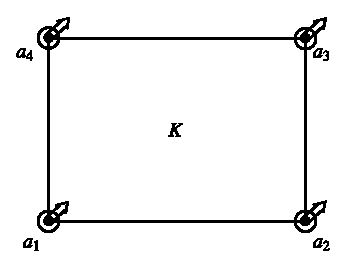
\includegraphics{figure/fig4.10.eps}
\caption{}\label{chap4-fig4.10}
\end{figure}

Let $P_{K}=Q_{3}$, the degrees of freedom being given by
$$
\sum_{K}=\left\{p(a_{i}),\frac{\p p}{\p x_{1}}(a_{i}),\ \frac{\p p}{\p
  x_{2}}(a_{i}),\ \frac{\p^{2}p}{\p x_{1}\p x_{2}}(a_{i}),\ 1\leq
i\leq 4\right\}.
$$

Show that $\sum_{K}$ determines uniquely a polynomial $p\in Q_{3}$ (a
double dotted arrow indicates that the mixed second derivative is a
degree of freedom). Show also that in this case $V_{h}\subset
C^{1}(\overline{\Omega})$. 
\end{exercise}

So far, we have verified requirements (i) and (ii) mentioned at the
beginning of this Section. Let us now examine requirement (iii), which
will be fulfilled by a ``canonical'' choice for the basis
functions. Let $\sum_{h}$ be the set of degrees of freedom of the
space $V_{h}$ derived in an obvious way from the sets $\sum_{K}$,
$K\in \mathfrak{k}_{h}$; Examples of such sets $\sum_{h}$ have been
given for $n$-simplices of type\pageoriginale $(k)$ and for Argyris
triangles. Then if
$$
\sum_{h}=\left\{\varphi_{jh},1\leq j\leq M\right\},
$$
we let the basis functions $w_{j}$, $1\leq j\leq M$, be those
functions in the space $V_{h}$ which satisfies
$$
\varphi_{i}(w_{j})=\delta_{ij},\ 1\leq i\leq M.
$$

Then it is easily seen that this choice will result in functions with
``small'' support: in Fig.~\ref{chap4-fig4.11}, we have represented
there types of supports encountered in this fashion, depending upon
the position of the node associated
\begin{figure}[H]
\centering
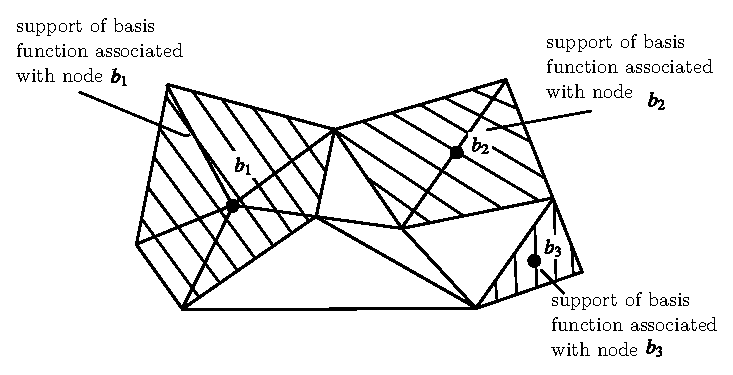
\includegraphics[scale=.9]{figure/fig4.11.eps}
\caption{}\label{chap4-fig4.11}
\end{figure}
\noindent
with the degree of freedom.

